\begin{definition}[Bloco $n$-dimensional]
  Um \textbf{bloco} $n$-dimensional $A\subseteq\mathbb{R}^{n}$ é o produtoo cartesiano
  \begin{align*}
    A=\prod_{i=1}^{n}[a_i,b_i]=[a_1,b_1]\times\cdots\times[a_n,b_n].
  \end{align*}
  de $n$ intervalos compactos $[a_i,b_i]$ (com $a_i\neq b_i$), chamados \textbf{arestas do bloco}. 
\end{definition}
\begin{definition}[Bloco aberto]
  O produto cartesiano
  \begin{align*}
    A=\prod_{i=1}^{n}(a_i,b_i).
  \end{align*}
  dos intervalos abertos $(a_i,b_i)$ chama-se \textbf{bloco $n$-dimensional aberto}. 
\end{definition}
\begin{definition}[Cubo]
  Quando todas as arestas do bloco $A$ tem o mesmo comprimento $l=b_i-a_i$ para todo $i$, diz-se que $A$ é um \textbf{cubo} $n$-dimensional. 
\end{definition}
\begin{definition}[Face]
  Uma face do bloco
  \begin{align*}
    A=\prod_{i=1}^{n}[a_i,b_i].
  \end{align*}
  é um conjunto do tipo
  \begin{align*}
    F=\prod_{i=1}^{n}L_i.
  \end{align*}
  Onde para cada $i$ ten-se uma das seguintes opções
  \begin{itemize}
    \item $L_i=\{a_i\}$.
    \item $L_i=\{b_i\}$.
    \item $L_i=[a_i,b_i]$.
  \end{itemize}
  Diz-se que a face $F$ tem \textbf{dimensão} $r$ quando exatamente $r$ dos fatores $L_i$ são iguais a $[a_i,b_i]$. 
\end{definition}
\begin{example}
  Seja $A=[0,1]\times[0,2]\times[0,3]$, logo você pode tomar $L_1=[0,1], L_2=[0,2]$ e $L_3=\{3\}$, então $F=L_1\times L_2\times L_3$ é uma face de $A$ e $F$ tem dimensão $2$. 
\end{example}
\begin{definition}[Vértices]
  As faces de dimensão $0$, i.é, os pontos da forma $v=(c_1,\cdots,c_2)$ com $c_i=a_i$ ou $c_i=b_i$ para cada $i=1,\cdots,n$ são chamados \textbf{vértices} do bloco. 
\end{definition}
\begin{definition}[Volúmen]
  O \textbf{vóume} $n$-dimensional do bloco $A=\prod_{i=1}^{n}[a_i,b_i]$ é o produto dos comprimentos das aristar, isto é
  \begin{align*}
    Vol(A)=\prod_{i=1}^{n}b_i-a_i.
  \end{align*}
\end{definition}
\begin{definition}[Partição]
  Uma partição do bloco $A=\prod_{i=1}^{n}[a_i,b_i]$ é o produto cartesiano
  \begin{align*}
    P=P_1\times P_2\times\cdots\times P_n.
  \end{align*}
  Onde cada $P_i$ é partiçã do intervalo $[a_i,b_i]$, i.é,
  \begin{align*}
    P_i=\{T_{i,0},T_{i,1},\cdots,T_{i,k_i}\},
  \end{align*}
  com $a_i=T_{i,0}<T_{i,1}<\cdots<T_{i,k_i}=b_i$.
\end{definition}
\begin{example}
  Suponha $A=[0,2]\times [-2,0]$, logo se tiramos
  \begin{align*}
    P_1&=\{0,1,2\}.\\
    P_2&=\{-2,-1,-0.5,0\}.
  \end{align*}
  Temos que uma partição $P$ do bloco $A$ é
  \begin{align*}
    P&=P_1\times P_2,\\
    &=\{(0,-2),(0,-1),(0,-0.5),(0,0)\\
    &\phantom{=-  }(1,-2),(1,-1),(1,-0.5),(1,0)\\
    &\phantom{=-  }(2,-2),(2,-1),(2,-0.5),(2,0)\}.
  \end{align*}
  \begin{center}
    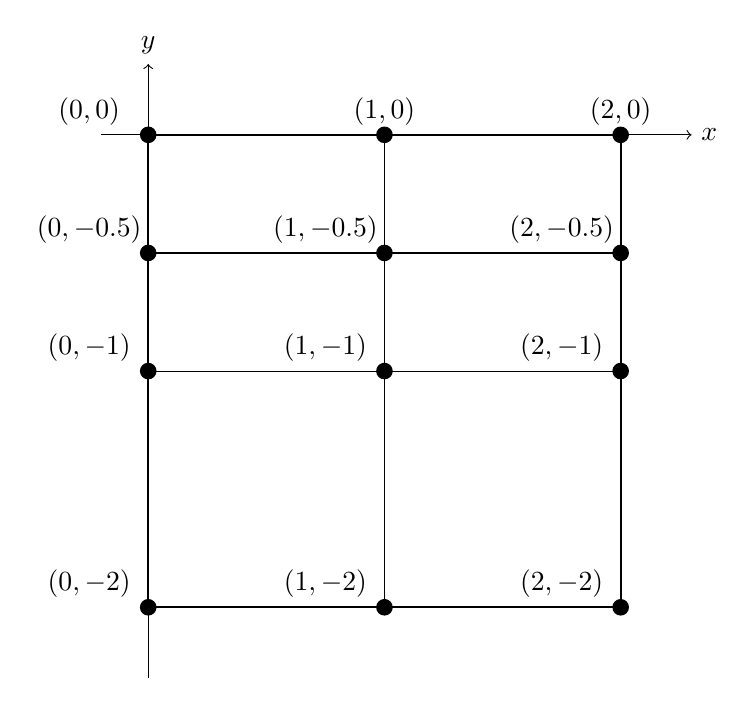
\begin{tikzpicture}[scale=3]

% Ejes
\draw[->] (-0.2,0) -- (2.3,0) node[right] {$x$};
\draw[->] (0,-2.3) -- (0,0.3) node[above] {$y$};

% Rectángulo A
\draw[thick] (0,-2) rectangle (2,0);

% Líneas de la partición en x
\draw (1,-2) -- (1,0);

% Líneas de la partición en y
\draw (0,-1) -- (2,-1);
\draw (0,-0.5) -- (2,-0.5);

% Puntos de la partición
\foreach \x in {0,1,2} {
    \foreach \y in {-2,-1,-0.5,0} {
        \fill (\x,\y) circle (0.5pt);
    }
}

% Puntos
\fill (0,0) circle (1pt);
  \node[above] at (-0.25,0) {$(0,0)$};

\fill (1,0) circle (1pt);
  \node[above] at (1,0) {$(1,0)$};

\fill (2,0) circle (1pt);
  \node[above] at (2,0) {$(2,0)$};

\fill (0,-0.5) circle (1pt);
  \node[above] at (-0.25,-0.5) {$(0,-0.5)$};

\fill (1,-0.5) circle (1pt);
  \node[above] at (0.75,-0.5) {$(1,-0.5)$};

\fill (2,-0.5) circle (1pt);
  \node[above] at (1.75,-0.5) {$(2,-0.5)$};

\fill (0,-1) circle (1pt);
  \node[above] at (-0.25,-1) {$(0,-1)$};

\fill (1,-1) circle (1pt);
  \node[above] at (0.75,-1) {$(1,-1)$};

\fill (2,-1) circle (1pt);
  \node[above] at (1.75,-1) {$(2,-1)$};

\fill (0,-2) circle (1pt);
  \node[above] at (-0.25,-2) {$(0,-2)$};

\fill (1,-2) circle (1pt);
  \node[above] at (0.75,-2) {$(1,-2)$};

\fill (2,-2) circle (1pt);
  \node[above] at (1.75,-2) {$(2,-2)$};

\end{tikzpicture}
  
  \end{center}
\end{example}
\begin{definition}[Refinamento]
  Diz-se que a partição $Q=Q_1\times\cdots\times Q_n$ \textbf{refina} a partição $P$ quando $P\subseteq Q$, ou seja, $P_i\subseteq Q_i$ para todo $i=1,\cdots,n$. 
\end{definition}
\begin{note}
  A partição $P$ decompõe bloco $A$ numa reunião de sub-blocos $B=I_1\times I_2\times\cdots\times I_n$. Onde cada $I_j$ é um intervalo da partição $P_j$ de $[a_j,b_j]$. Estos sub-blocos $B\subseteq A$ chama-se os \textbf{blocos da partição} $P$ e escreve-se $B\in P$.\\
  Note que se $Q$ refina $P$, então dado $P^{\prime}\in P$, temos que 
  \begin{align*}
    P^{\prime}=\bigcup_{\substack{P^{\ast}\in Q\\P^{\ast}\subseteq P^{\prime}}}P^{\ast}.
  \end{align*}
\end{note}
\begin{theorem}[Propriedade fundamental]
  Dada a partição $P=P_1\times\cdots\times P_n$ do bloco $A$ como o comprimento $b_i-a_i$ de cada aresta de $A$ é a soma dos comprimentos dos intervalos da partição $P_i$, segue-se que
  \begin{align*}
    Vol(A)=\sum_{B\in P}Vol(B).
  \end{align*}
\end{theorem}
\begin{proof} 
  Seja $P_i=\{T_{i,0},\cdots,T_{i,k_{i}}\}$ uma partição. Então os intervalos $P_i=[T_{i,j-1},T_{i,j}]$ com comprimento $\Delta T_{i,j}=T_{i,j}-T_{i,j-1}$ temos que
  \begin{align*}
    Vol(A)=\prod_{i=1}^{n}(b_i-a_i)=&\prod_{i=1}^{n}\left( \sum_{j=1}^{k_i}\Delta T_{i,j} \right)\\
    =&\sum_{j_1=1}^{k_1}\cdots\sum_{j_n=1}^{k_n}\Delta T_{1,j_1}\cdots\Delta T_{n,j_n}\\
    =&\sum_{j_1=1}^{k_1}\cdots\sum_{j_n=1}^{k_n}Vol(B_{j_1\cdots j_n})\\
    =&\sum_{B\in P}Vol(B).
  \end{align*}
\end{proof}
\begin{lemma}[Existencia de refinamento común]\label{lema:refinamento-comun}
  Se $P$ e $Q$ são partições do bloco $A$, então existe uma partição $R$ de $A$ que refina simultaneamente $P$ e $Q$.\\
  Uma delas é
  \begin{align*}
    R=\prod_{i=1}^{n}P_i\cup Q_i.
  \end{align*}
\end{lemma}
\begin{proof} 
  Basta tomar a união dos pontos de $P_i$ e $Q_i$ em cada coordenada e formar o produto cartesiano. 
\end{proof}
\begin{definition}[Somas inferior e superior]
  Seja $f:A\to\mathbb{R}$ uma função real limitada no bloco $n$-dimensional $A$. Existem $m,M\in\mathbb{R}$ tais que
  \begin{align*}
    m\leq f(x)\leq M,\quad\text{para todo }x\in A.
  \end{align*}
  Logo, dada uma partição $P$ do bloco $A$, para cada bloco $B\in P$ indiquemos
  \begin{align*}
    m_{B}=\inf_{x\in B}f(x),\,M_B=\sup_{x\in B}f(x),\,w_{B}=M_B-m_B.
  \end{align*}
  Agora, definimos a \textbf{soma inferior} $s(f,P)$ e a \textbf{soma superior} $S(f,P)$ da função $f$ relativamente a partição $P$ pondo
  \begin{align*}
    s(f,P)=\sum_{B\in P}m_B Vol(B).\\
    S(f,P)=\sum_{B\in P}M_B Bol(B).
  \end{align*}
\end{definition}
\begin{note}
  Como $m_b\leq M_B$ temos que
  \begin{align*}
    s(f,P)\leq S(f,P).
  \end{align*}
\end{note}
\begin{lemma}\label{lema:particao-refinada-somas}
  Se uma partição $Q$ refina a partição $P$, então
  \begin{align*}
    s(f,P)\leq S(f,Q)\,\text{ e }\,S(f,Q)\leq S(f,P).
  \end{align*}
\end{lemma}
\begin{proof} 
  Suponha que $Q$ refina $P$ temos que dado $B\in P$, se $B^{\ast}\in Q$ e $B^{\ast}\subseteq B$ se cumpre que 
  \begin{align*}
    m_{B}=\inf_{x\in B}f(x)\leq \inf_{x\in B^{\ast}}f(x)=m_{B^{\ast}}.
  \end{align*}
  Logo
  \begin{align*}
    s(f,P)=\sum_{B\in P}m_BVol(B)=\sum_{B\in P}m_B\sum_{\substack{B^{\ast}\in Q\\ B^{\ast}\subseteq B}}Vol(B^{\ast})\leq\sum_{B\in P}\sum_{\substack{B^{\ast}\in Q\\ B^{\ast}\subseteq B}}m_{B^{\ast}}Vol(B^{\ast})=s(f,Q).
  \end{align*}
  A prova da soma superior é semelhante.
\end{proof}
\begin{lemma}\label{lema:somainferior-somasuperior}
  Para quaisquer partições $P$ e $Q$ do bloco $A$, tem-se
  \begin{align*}
    s(f,P)\leq S(f,Q).
  \end{align*}
\end{lemma}
\begin{proof}
  Pelo lema \ref{lema:refinamento-comun} sabemos que existe uma partição $R$ de $A$ que refina simultaneamente $P$ e $Q$, logo pelo lema \ref{lema:particao-refinada-somas} temos que
  \begin{align*}
    s(f,P)\leq s(s,R)\leq S(f,R)\leq S(f,Q).
  \end{align*}
\end{proof}
\begin{definition}[Integral inferior e superior]
  Dada a função limitada $f:A\to\mathbb{R}$, definimos a \textbf{integral inferior} de $f$ em $A$ como 
  \begin{align*}
    \underline{\int}_{A}f(x)\,dx=\sup_{P}s(f,P).   
  \end{align*}
  Da mesma maneira, definimos a \textbf{integral superior} de $f$ em $A$ como 
  \begin{align*}
    \overline{\int}_{A}f(x)\,dx=\inf_{P}S(f,P).   
  \end{align*}
\end{definition}
\begin{note}
  Note que pelo lema \ref{lema:somainferior-somasuperior} temos que dada $P$ partição se cumpre que
  \begin{align*}
    s(f,P)\leq \underline{\int}_{A}f(x)\,dx\,\text{ e }\,\overline{\int}_{A}f(x)\,dx\leq S(f,P).
  \end{align*}
  Além disso,
  \begin{align*} 
    mVol(A)\leq \underline{\int}_{A}f(x)\,dx\,\text{ e }\,\overline{\int}_{A}f(x)\,dx\leq MVol(B).
  \end{align*}
\end{note}
\begin{definition}[Integral]
  Diz-se que a função $f:A\to\mathbb{R}$ é \textbf{integrável} no bloco $n$-dimensional $A$ quando a integral superior e a integral inferior são iguales, denotamos este número por
  \begin{align*}
    \int_{A}f(x)\,dx=\underline{\int}_{A}f(x)\,dx=\overline{\int}_{A}f(x)\,dx.
  \end{align*}
  Chamamos este numero como a \textbf{integral} de $f$ no bloco $A$. 
\end{definition}
\begin{theorem}
  A fim de que a função limitada $f:A\to\mathbb{R}$ seja integrável no bloco, $A\subseteq\mathbb{R}^{m}$ é necessario e suficiente que para todo $\epsilon>0$ existe uma partição $P$ de $A$ tal que
  \begin{align*}
    S(f,P)-s(f,P)<\epsilon.
  \end{align*}
\end{theorem}
